\begin{figure*}[t]
    \centering
    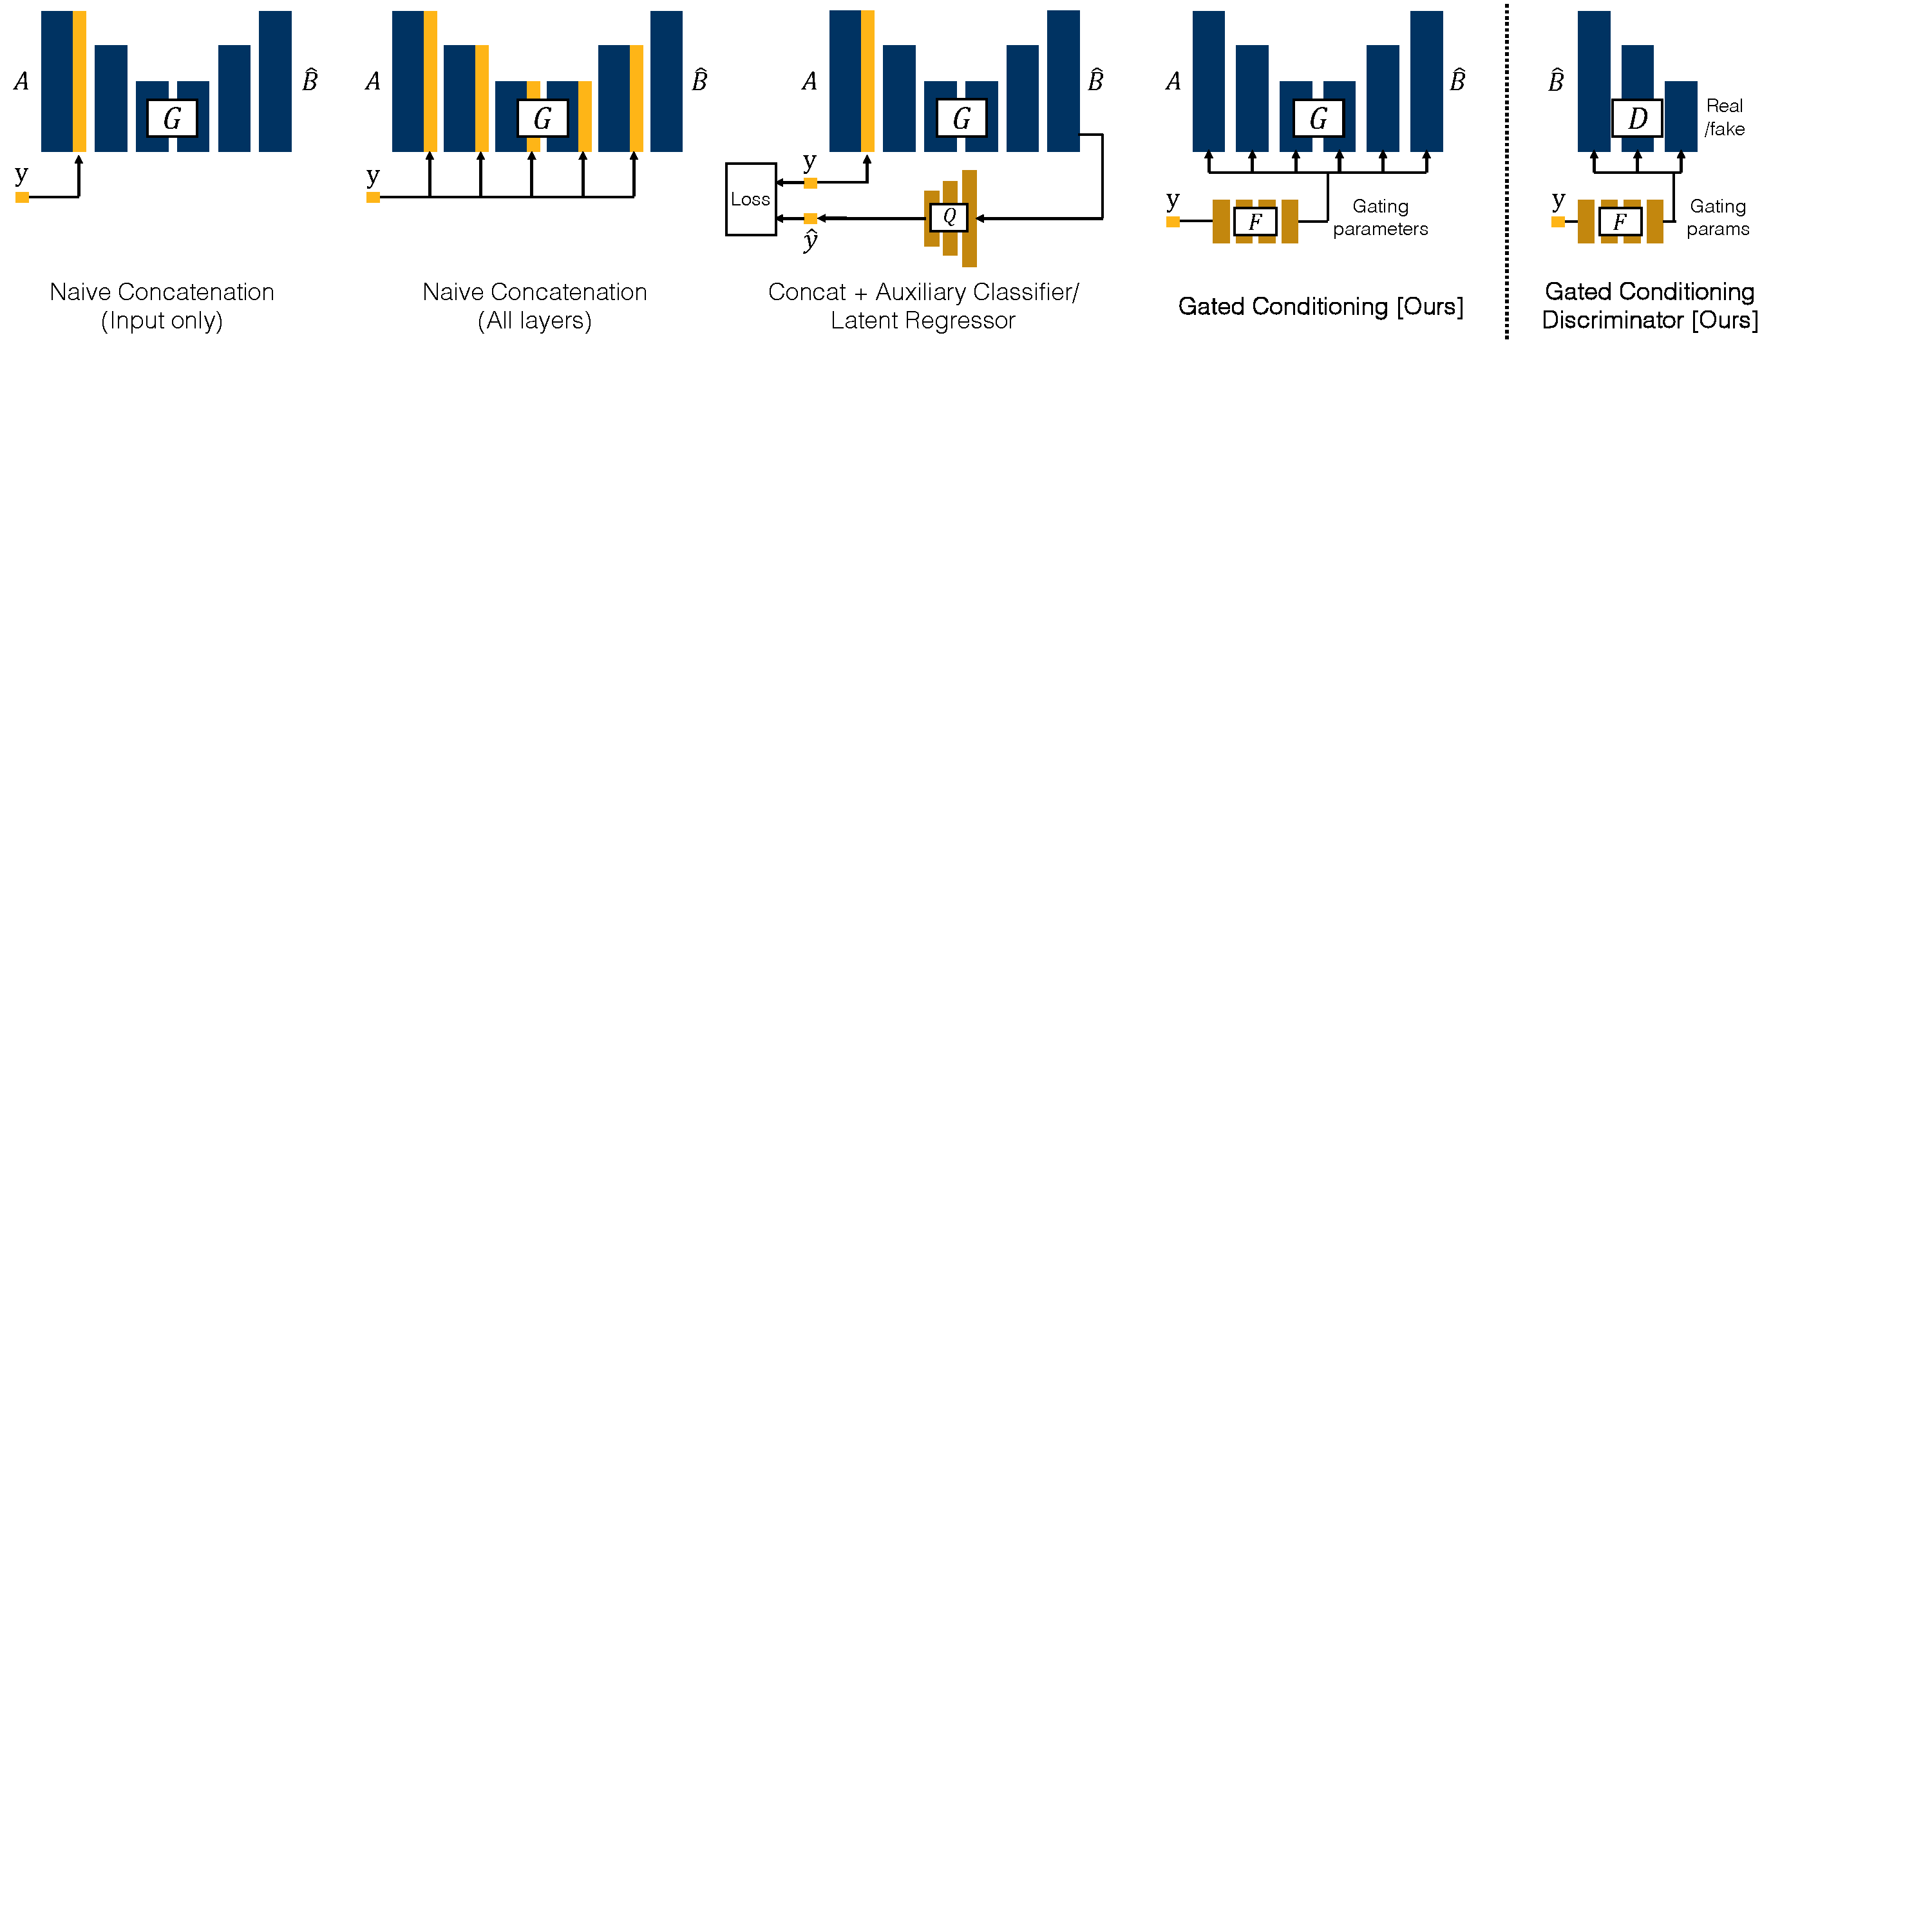
\includegraphics[width=\linewidth]{paper_images/arch_inject.pdf}
    \caption{{\bf Conditioning injection variants.} Conditioning information can be incorporated naively in a generator architecture through simple concatenation in {\bf (left)} the input layer only or {\bf (mid-left)} in all layers. {\bf (Mid-right)} The network can be further encouraged to use the conditioning through a learned network, either a classification objective for categorical conditioning~\cite{XX,XX} or a regression objective for continuous conditioning. {\bf (Right)} We investigate training a network on the conditioning signal, which predicts parameters which are used to guide softly-gated units in the main network. Note that these options -- concatenation, auxiliary classifier/latent regressor, and gated conditioning -- can also be correspondingly applied to a discriminator.\label{fig:arch-inj} }
    % \vspace{-4mm}
\end{figure*}

% ***** RZ *****
\section{Methods}

We consider image-to-image translation problems, mapping input image $A \in \mathds{R}^{H\times W\times 3}$ to output $B \in \mathds{R}^{H\times W\times 3}$, with the benefit of a conditioning vector $y \in \mathds{R}^{D}$. We learn this mapping with $L$-layer generator $\widehat{B}=\mathcal{G}(A,y)$. We refer to the feature map at each channel as $x_l\in \mathds{R}^{H_l\times W_l\times C_l}$, where $H_l \times W_l$ is the spatial size of the feature map, and $C_l$ is the number of channels in the layer. The total channels in the network is $C = \sum_l C_l$. The conditioning vector $y$ can be categorical, expressed as a 1-hot vector, or a continuous vector.
% , ground truth output $B \in \mathds{R}^{H\times W\times 3}$, generator $\mathcal{G}$, output $\widehat{B}=\mathcal{G}(A,y)$.

\subsection{Conditioning injection variants}

The structure of the generator plays a critical role in the effectiveness of the conditioning. We systematically explore several variants, as illustrated in Figure~\ref{fig:arch-inj}.

\paragraph{Naive concatenation (input only)} The most straightforward method for incorporating the conditioning is to spatially replicate the vector into a tensor of appropriate size, and concatenate it to the input layer~\cite{XX,XX}.

\paragraph{Naive concatenation (all layers)} A potential weakness is the large distance between the conditioner and the output, which can lead to the generator ignoring the conditioner during learning. A possible solution is to simply concatenate the conditioner into every layer. This has been previously explored in ~\cite{zhu2017toward}.

\paragraph{Recovering the conditioner} An alternative is to encourage the use of the contioner through optimization. One can add a hypernetwork, $Q$, charged with recovering the conditioner from the output $\widehat{B}$. A loss $\ell$ is added to the optimization between ground truth $y$ and predicted $\widehat{y}$. This term encourages the output to contain enough information about the conditioner. This approach has been explored in the classification setting with Auxiliary-Classifier GAN (ACGAN)~\cite{XX}, regression setting with InfoGAN~\cite{XX} and BiGAN (``latent regressor" model)~\cite{XX}, and is one half of the BicycleGAN model~\cite{zhu2017toward}.

\begin{figure*}[t]
    \centering
    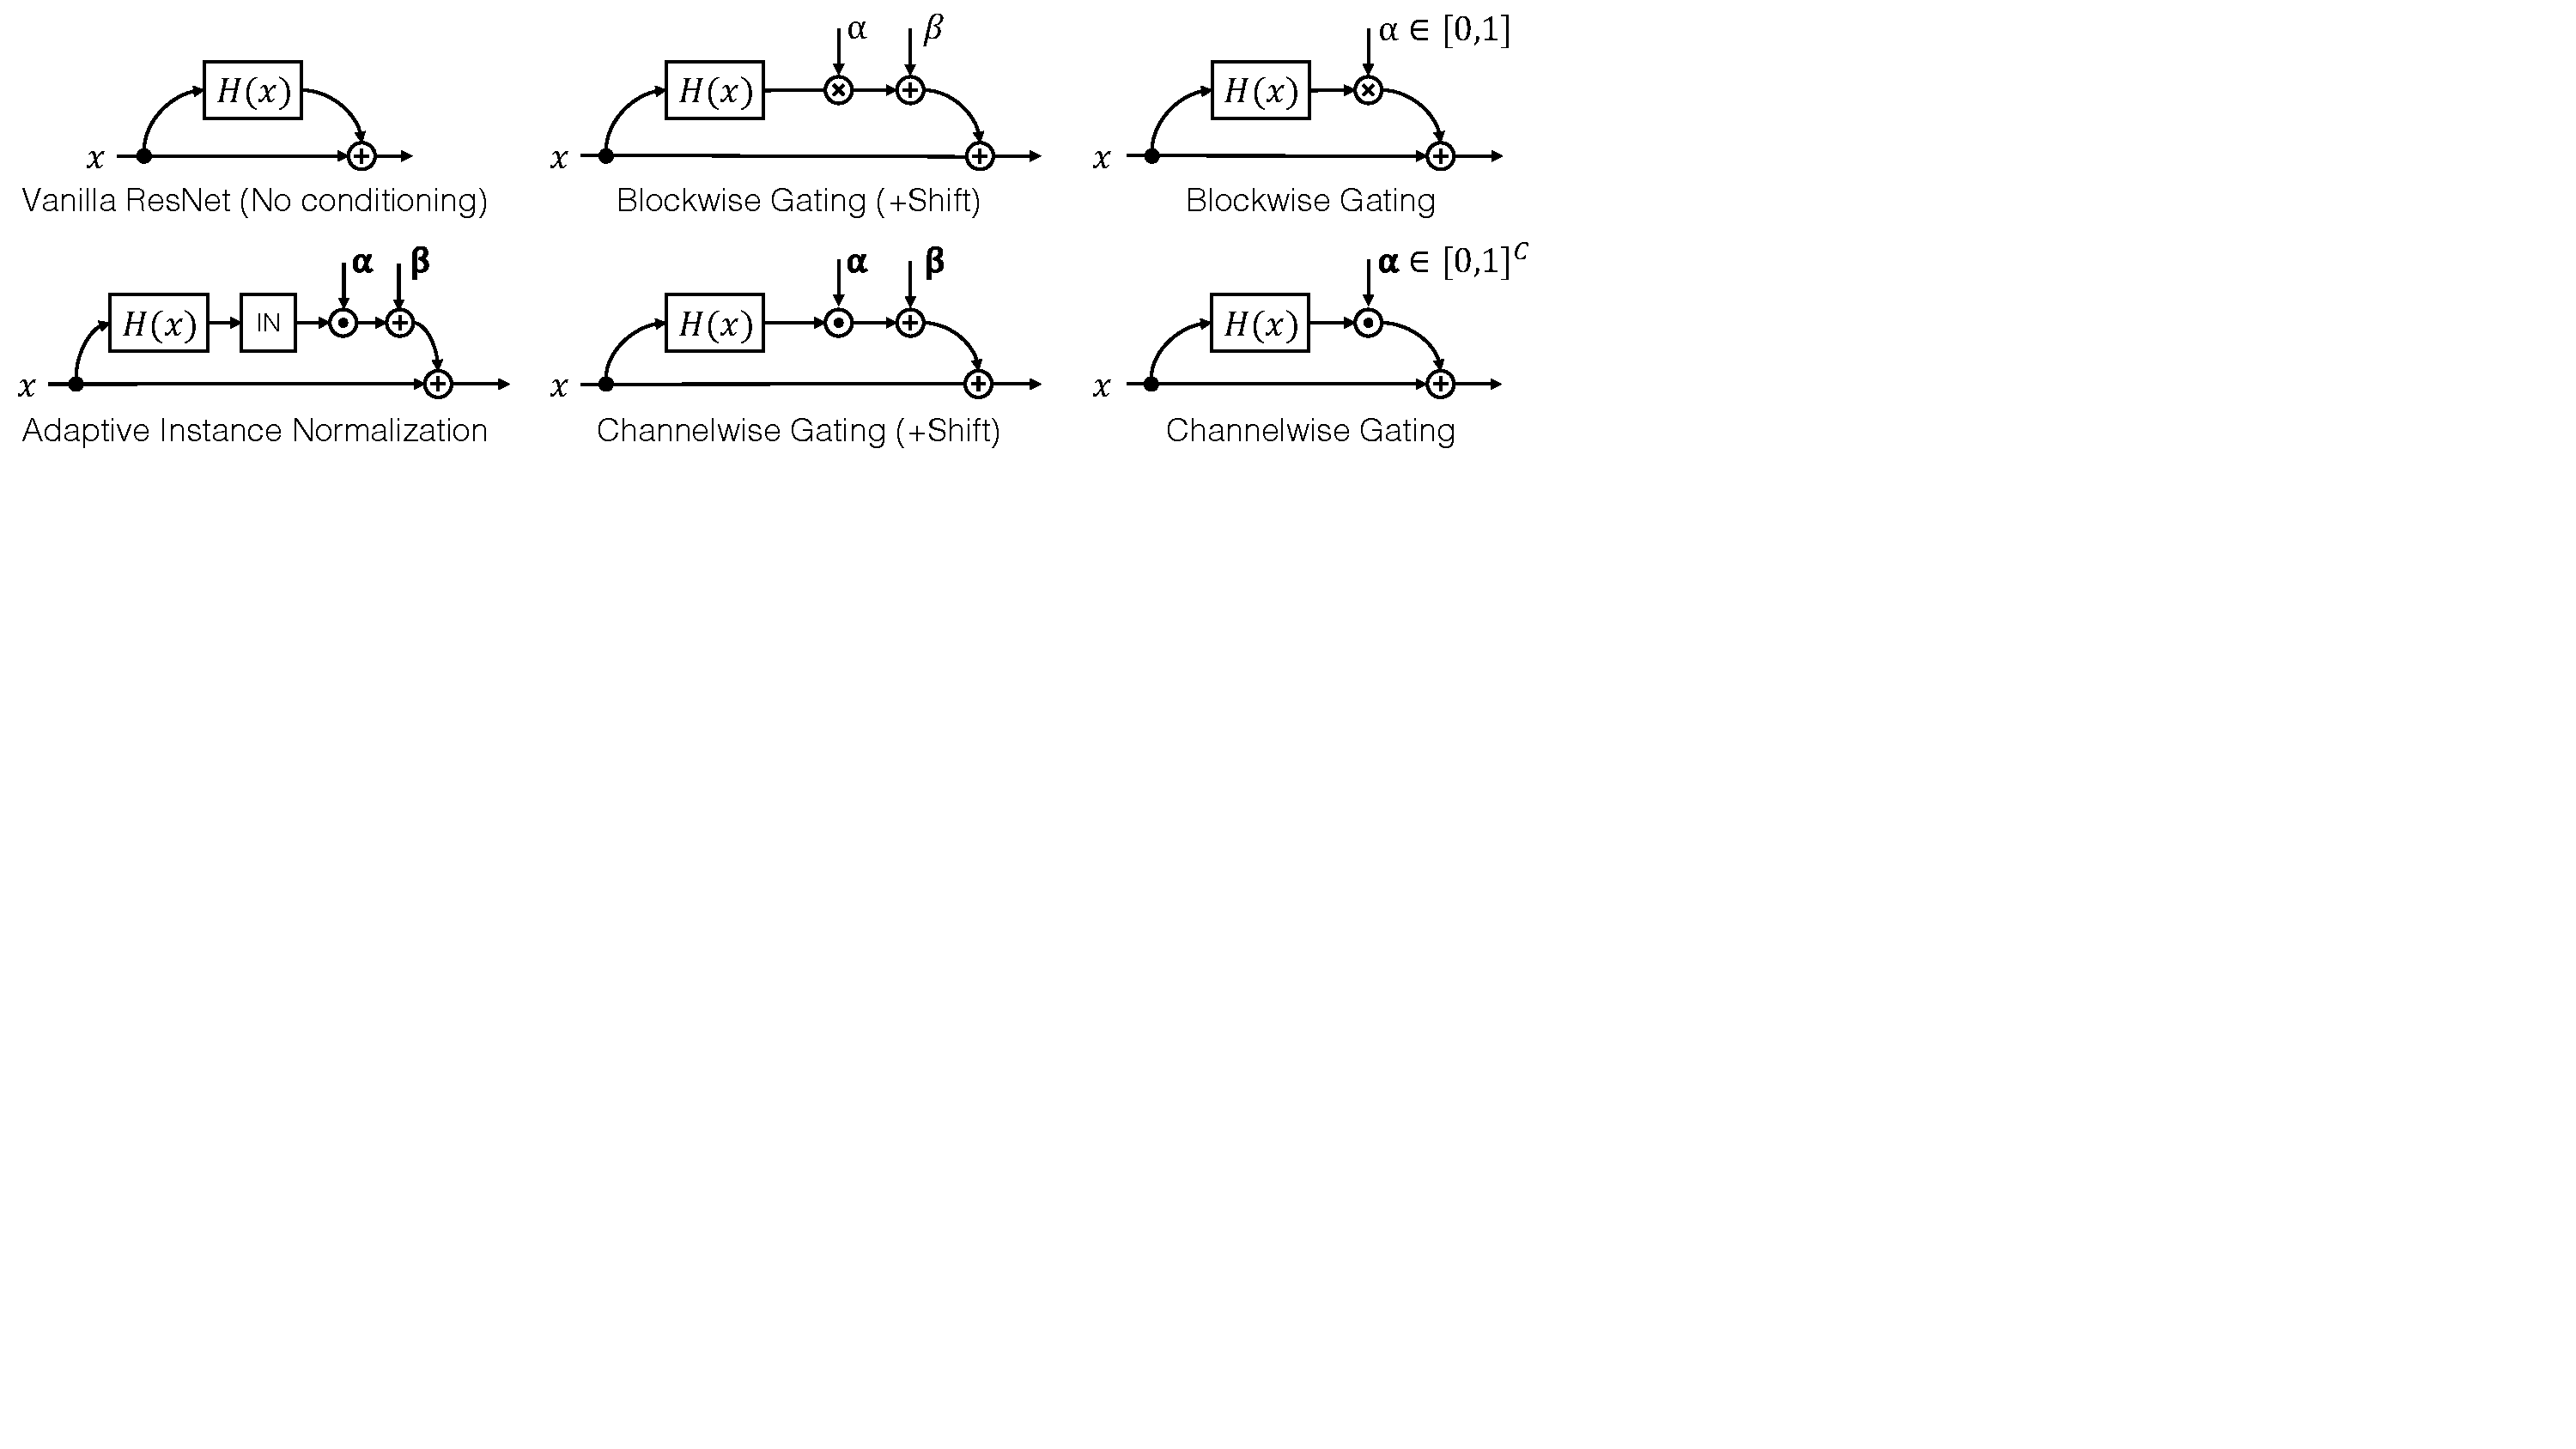
\includegraphics[width=\linewidth]{paper_images/arch_gate.pdf}
    \caption{{\bf Incorporating soft-gating into residual blocks.} {\bf (Top-left)} A ``vanilla" residual block without gated conditioning parameters modifies signal $x$ into $x+\mathcal{H}(x)$. {\bf (Top-mid)} The full $\mathcal{H}(x)$ block is softly-gated by scalar parameter $\alpha$. {\bf (Top-right)} Each channel is softly-gated by vector parameter $\mathbf{\alpha}$. {\bf (Bot-left)} Adaptive Instance Normalization applied after the whole residual operation involves both a scaling and a bias. {\bf (Bot-mid, Bot-right)} A bias can be added to either block-wise or channel-wise gating. We find that channel-wise gating (without added bias) to empirically produces the best results.\label{fig:arch-gate} }
    % \vspace{-4mm}
\end{figure*}

\paragraph{Proposed Soft-Gating for Generation} The methods above do not fundamentally modify the structure of the network. In a residual network, a feature tensor $x$ is modified by function $x+H(x)$.

% We now begin to describe our model which we call Gated Generative Adversarial Networks (GAN-Gate). It is primarily based on an interesting experiment whereby \cite{veit2016residual} showed that the residual networks behave as an ensemble of several shallower networks, and removing a few residual blocks at test time performed highly competitive to the original network itself. This implies that, perhaps, given a GAN architecture with residual blocks as its components, it is possible to {\em automatically} learn a mixture of shallower networks {\em conditioned} on the modes of the data distribution or the tasks we are interested in. This is exactly the objective that GAN-Gate achieves. More precisely, it automatically learns a mixture of shallower networks where each mixture component (a shallow network) is focused on generating data either from a mode or a task; depending on whether we are interested in {\em intraclass} or {\em interclass} variations. To this end, we first propose an architecture for GANs entirely based on residual blocks which is capable of generating highly competitive samples form image-to-image translation task compared to other baselines. Then, we propose to use a simple yet powerful {\em gating mechanism} over a subset of residual blocks where the gating automatically decides which blocks to {\em focus on} for a given condition. Note, this gating is learned automatically from the data. In the end, we also show that the gating mechanism provides an effective way to maximize mutual information in the {\em InfoGAN} objective, which otherwise was not possible.

Inspired by the incision experiments by Veit et al.~\cite{veit2016residual,veit2018adaptive}, we investigate the use of \textit{learned} gating, or incision, on the generator. There are multiple variants of this idea, which we illustrate in Figure~\ref{fig:arch-gate}. We begin by predicting an $\alpha$ using a learned network $F(y)$ for each layer of the network.

\begin{equation}
x + \mathbf{\alpha} H(x), \text{where } \alpha \in [0,1]
\end{equation}

If a class does not have use for a particular block, it can predict $\alpha$ close to zero, and effectively switch off the layer. Intuitively, during training, blocks within the main network can transform the image in various ways, and network $F$ can modulate such that the the ``right" blocks are selected.

We can apply the operation channel-wise as well, using a predicted vector $\alpha$. This provides additional degrees of freedom for network $F$, to choose to switch specific changes to channels ``on" or ``off".

\begin{equation}
x + \mathbf{\alpha} \odot H(x), \text{where } \odot \text{is channel-wise multiplication}
\end{equation}

We make the corresponding changes in the discriminator as well. Soft-gating has been explored by Veit et al.~\cite{veit2018adaptive} in a classification setting. Intuitively, this can enable the discriminator to select blocks which effectively judge whether generations are real or fake, conditioned on the class input.
% Via accurate gradients backpropagated to the generator it also enables the generator to generate class conditioned high resolution image samples.
Some blocks can be shared across regions in the conditioning vector, whereas other blocks can specialize for a given class.

We empirically find that channel-wise gating provides the strongest results. For completeness, we additionally explore incorporating shifting after the soft-gating, either block-wise using a scalar $\beta$ per layer, or channel-wise using a vector $\mathbf{\beta}$ per layer.

\paragraph{Scaling and shifting activation distributions} The soft-gating parameter and shifting bears resemblance to the Adaptive Instance Normalization (AdaIN) layer.

\begin{equation}
\text{AdaIn}(x, \alpha, \beta) = \alpha \big(\frac{x-\mu(x)}{\sigma(x)}\big)+\beta
\label{eqn:adain}
\end{equation}

The AdaIn layer is applied in between residual layers, and $\alpha$ is not constrained between $[0,1]$. The layer has previously been used to great success in style transfer~\cite{huang2017arbitrary} and multimodal image-to-image translation~\cite{XX}.

% \subsection{Improvement on InfoGAN}
\subsection{Improving the Effectiveness of InfoGAN}
\label{sec:infoGAN}
InfoGAN\cite{chen2016infogan} has shown impressive results in unconditional image generation where the objective is to maximize the mutual information between the generations $G(z,c;\theta_g)$ and the latent codes $c$, along with generating `real' looking samples. Intuitively, mutual information is maximized if different latent codes allow diverse generations, making the generation and the latent code dependent. However, in the conditional generation situation, where the condition $y$ is highly informative, for example an image, it has been empirically shown that irrespective of how much the noise $z$ or the latent code $c$ is being modified, InfoGAN still suffers from the {\em mode-collapse} issue\cite{ghosh2017multi}. Thus, fails to generate diverse generations for an extremely important and challenging task of image-to-image translation. For brevity, below we provide the objective function of the generator for the conditional variant of InfoGAN ($z$ removed to avoid clutter):
\begin{align}
\label{eq:infoGAN-gen}
\min_{\theta_g} \log (1 - D(G(y,c; \theta_g); \theta_d) - \lambda \; I (G(y,c; \theta_g), c)
\end{align}
%Note, since we only modify the generation process, the objectives of the Q-network and the discriminator is not being discussed here. 
Generally mode-collapse is the result of the following approximation $G(y,c; \theta_g) \approx G(y; \theta_g), \forall c$. Even though the mutual information term should make $G(y,c;\theta_g)$ and $c$ dependent, it turns out that this is not the case in practice. We advocate the objective function of InfoGAN, however, we hypothesize that the lack of participation of $c$ in the generation process does not allow it to make the generated samples and the latent codes dependent on each other. The gatings, however, resolves this issue by making $c$ an active part of the generation process. Also, from the well known {\em data processing inequality}, for any sequential transformation process (\eg feedforward neural networks) over a random variable $c \to f_1(c) \to f_2(f_1(c)) \to x$ (could be of any length); the dependence between $x$ and the transformed random variable decreases as the separation from $x$ increases. This implies $I(x, f_2(f_1(c)) \geq I (x, f_1(c) \geq I (x, c)$. Since the gating function brings $c$ closer to $G(y,c;\theta_g)$, it is straightforward to see that the above inequality implies $I_{Gate}(G(y,c;\theta_g), c) \geq I(G(y,c;\theta_g), c)$. Thus, gating allows the objective to maximize mutual information in a much more effective way than without it. We validate this experimentally by showing that just with gating, InfoGAN is able to produce diverse plausible samples for the image-to-image translation task, which otherwise was not possible.


\subsection{Network Architecture}

\paragraph{Skinny ResNet}

\paragraph{Encoder-Decoder} As a baseline, we test the encoder-decoder architecture from MUNIT~\cite{XX}. ...

% ***** RZ *****

% \paragraph{Architecture}

% \section{Gated Residual Block based Generator}
% Inspired by the incision experiments performed on the generator whereby removal of certain blocks led to the removal of particular modes from the data distribution, our model consists of a main network which is oblivious to the condition provided to the network, while another hypernetwork only receives the condition and has to predict which block should be used to what extent. More precisely, the $i^{th}$ residual block now receives an extra input $\alpha_i$ alongside the usual $x$ and the output of the gated residual block is $x+\alpha_i*f_i(x)$ rather than the standard $x+f_i(x)$. The $alpha_i$s are predicted via another hypernetwork which only receives the condition and has no idea about the input being received by the main block. The interpretation of the above is that if some block doesn't have to be used for a particular class then the hypernetwork can just choose the $alpha_i$ close to 0 and effectively that block is switched off. The intuition is that the hypernetwork has to first understand the transformations that the different residual blocks in the generator are learning, then start modulating it such that conditioned on the class the required blocks are chosen to the right extent such that the resulting sequence of transformations corresponds to realistic images from that particular class. Its related to FILM \cite{perez2017film} albeit it does feature wise transform and has to predict more parameters than a single number per block. \figref{fig:gru_gen} illustrates the concept in the setting of the conditional generator. Some other extensions such as affine gating per residual block and channel wise gating with its affine counterpart exists as well apart from the well known Adaptive Instance Normalization \cite{huang2017arbitrary} . The varied forms of gating could be applied to the Infogan setup with the gate prediction block receives the randomly sampled latent as input to decide the gates on the various blocks while the Q network trying to reconstruct back the latent that was passed.
 
% \section{Gated Residual Block based Discriminator}

% Based on a similar principle as the Generator, the Discriminator can also be equipped with gated residual blocks whereby each residual block would compute $x+\alpha_i*f_i(x)$ in place of the standard $x+f_i(x)$ where each $alpha_i$ is predicted by another hypernetwork which gets the condition that which class is the network currently judging for real/fake. Its intriguing that with just the class information the hypernetwork is able to select blocks which effectively guide the discriminator to judge whether its real/fake conditioned on the class. Via accurate gradients backpropagated to the generator it also enables the generator to generate class conditioned high resolution image samples. Intuitively, the discriminator distributes some common functions between the different classes to some of these shared residual blocks which are activated for all classes while the rest of the transformations it distributes in a non-overlapping manner to some specific residual blocks of the discriminator network. Such a concept can not only be used for the discriminator but in many settings where the conditioning variable is known, for example some plausible applications can be the Q network in InfoGAN\cite{chen2016infogan} or the Conditional Inference Network in a CVAE \cite{sohn2015learning}. \figref{fig:gru_dis} illustrates the concept in the setting of the conditional discriminator. Some other extensions such as affine gating per residual block and channel wise gating with its affine counterpart exists as well apart from Adaptive Instance Normalization(AdaIN) \cite{huang2017arbitrary}

% \section{GAN-Gate}
% We now begin to describe our model which we call Gated Generative Adversarial Networks (GAN-Gate). It is primarily based on an interesting experiment whereby \cite{veit2016residual} showed that the residual networks behave as an ensemble of several shallower networks, and removing a few residual blocks at test time performed highly competitive to the original network itself. This implies that, perhaps, given a GAN architecture with residual blocks as its components, it is possible to {\em automatically} learn a mixture of shallower networks {\em conditioned} on the modes of the data distribution or the tasks we are interested in. This is exactly the objective that GAN-GATE achieves. More precisely, it automatically learns a mixture of shallower networks where each mixture component (a shallow network) is focused on generating data either from a mode or a task; depending on whether we are interested in {\em intraclass} or {\em interclass} variations. To this end, we first propose an architecture for GANs entirely based on residual blocks which is capable of generating highly competitive samples form image-to-image translation task compared to other baselines. Then, we propose to use a simple yet powerful {\em gating mechanism} over a subset of residual blocks where the gating automatically decides which blocks to {\em focus on} for a given condition. Note, this gating is learned automatically from the data. In the end, we also show that the gating mechanism provides an effective way to maximize mutual information in the {\em InfoGAN} objective, which otherwise was not possible.

% \subsection{Residual Blocks based GAN Architecture}
\label{sec:resnet-architecture}
% \pd{Brief overview of our architecture?}
% \subsection{Gated Residual Blocks and its Variants}
% \label{sec:gated-resnet}
% \pd{talk about gating and its variants. relation with FilM etc? Point to Richard's figure and provide some intuitions}
% \subsection{Improving the Effectiveness of InfoGAN}
% \label{sec:infoGAN}
% InfoGAN\cite{chen2016infogan} has shown impressive results in unconditional image generation where the objective is to maximize the mutual information between the generations $G(z,c;\theta_g)$ and the latent codes $c$, along with generating `real' looking samples. Intuitively, mutual information is maximized if different latent codes allow diverse generations, making the generation and the latent code dependent. However, in the conditional generation situation, where the condition $y$ is highly informative, for example an image, it has been empirically shown that irrespective of how much the noise $z$ or the latent code $c$ is being modified, InfoGAN still suffers from the {\em mode-collapse} issue\cite{ghosh2017multi}. Thus, fails to generate diverse generations for an extremely important and challenging task of image-to-image translation. For brevity, below we provide the objective function of the generator for the conditional variant of InfoGAN ($z$ removed to avoid clutter):
% \begin{align}
% \label{eq:infoGAN-gen}
% \min_{\theta_g} \log (1 - D(G(y,c; \theta_g); \theta_d) - \lambda \; I (G(y,c; \theta_g), c)
% \end{align}
% %Note, since we only modify the generation process, the objectives of the Q-network and the discriminator is not being discussed here. 
% Generally mode-collapse is the result of the following approximation $G(y,c; \theta_g) \approx G(y; \theta_g), \forall c$. Even though the mutual information term should make $G(y,c;\theta_g)$ and $c$ dependent, it turns out that this is not the case in practice. We advocate the objective function of InfoGAN, however, we hypothesize that the lack of participation of $c$ in the generation process does not allow it to make the generated samples and the latent codes dependent on each other. The gatings, however, resolves this issue by making $c$ an active part of the generation process. Also, from the well known {\em data processing inequality}, for any sequential transformation process (\eg feedforward neural networks) over a random variable $c \to f_1(c) \to f_2(f_1(c)) \to x$ (could be of any length); the dependence between $x$ and the transformed random variable decreases as the separation from $x$ increases. This implies $I(x, f_2(f_1(c)) \geq I (x, f_1(c) \geq I (x, c)$. Since the gating function brings $c$ closer to $G(y,c;\theta_g)$, it is straightforward to see that the above inequality implies $I_{Gate}(G(y,c;\theta_g), c) \geq I(G(y,c;\theta_g), c)$. Thus, gating allows the objective to maximize mutual information in a much more effective way than without it. We validate this experimentally by showing that just with gating, InfoGAN is able to produce diverse plausible samples for the image-to-image translation task, which otherwise was not possible.
\subsection{Interclass Variability using GAN-GATE}
\label{sec:interclass}
%As discussed in Section~\ref{sec:infoGAN}, the InfoGAN objective along with the gating for the generator effectively captures the intraclass variability. 
Since intraclass variability is something that requires automatic disentanglement, as the ground-truth for this is not provided (modes unknown), an InfoGAN type objective is a suitable choice for this (see Section~\ref{sec:infoGAN}). However, for the interclass variability, the ground-truth already provides the task or the class id (\eg, `cat', `dog' \etc) during training. Therefore, there is no need for the network to automatically disentangle them. This avoids the requirement of the mutual information component. To this end, we use gating in both generator and the discriminator to capture interclass variability. 

The gating in the generator, similar to the arguments provided in Section~\ref{sec:infoGAN}, makes the generation process highly dependent on the class condition. However, providing class-conditional gating for the discriminator enforces it to learn a particular subnetwork for a task to decide whether it is real or fake. This, in turn, via accurate gradient back-propagation provides informative gradients to the generator that enables it to generate class conditioned high resolution image samples. Intuitively, the discriminator distributes some common functions between the different classes to some of these shared residual blocks which are activated for all classes while the rest of the transformations it distributes in a non-overlapping manner to some specific residual blocks of the discriminator network. Such a concept can not only be used for the discriminator but in many settings where the conditioning variable is known, for example some plausible applications can be the Q network in InfoGAN\cite{chen2016infogan} or the Conditional Inference Network in a CVAE \cite{sohn2015learning}. \figref{fig:gru_dis} illustrates the concept in the setting of the conditional discriminator. Some other extensions such as affine gating per residual block and channel wise gating with its affine counterpart exists as well apart from Adaptive Instance Normalization(AdaIN) \cite{huang2017arbitrary}.


\begin{table}[ht]
\caption{Resblock} % title of Table
\centering % used for centering table
\begin{tabular}{c} % centered columns (4 columns)
\hline\hline %inserts double horizontal lines
F(x)\\%heading
\hline % inserts single horizontal line
Linear(4,4)\\ % inserting body of the table
ReLU() \\
Linear(4,4) \\
\hline %inserts single line
\end{tabular}
\label{table:resblock} % is used to refer this table in the text
\end{table}


\begin{table}[ht]
\caption{Generator} % title of Table
\centering % used for centering table
\begin{tabular}{c c} % centered columns (4 columns)
\hline\hline %inserts double horizontal lines
layer & num layers\\%heading
\hline % inserts single horizontal line
Linear(10,4) & 1\\ % inserting body of the table
ResBlock & 16 \\
Linear(4,1) & 1 \\
\hline %inserts single line
\end{tabular}
\label{table:1d_G} % is used to refer this table in the text
\end{table}

\begin{table}[ht]
\caption{Discriminator} % title of Table
\centering % used for centering table
\begin{tabular}{c c} % centered columns (4 columns)
\hline\hline %inserts double horizontal lines
layer & num layers\\%heading
\hline % inserts single horizontal line
Linear(1,4) & 1\\ % inserting body of the table
ResBlock & 16 \\
Linear(4,1) & 1 \\
Sigmoid & 1 \\
\hline %inserts single line
\end{tabular}
\label{table:1d_D} % is used to refer this table in the text
\end{table}
